%% 1
Burger's equation can be solved numerically using the Lax and Lax-Wendroff scheme.
The Burger equation is given by
\begin{equation}
\frac{\partial \rho}{\partial t} = \frac{\partial (v \rho)}{\partial x}
\end{equation}
where
\begin{equation}
v(\rho) = v_m \left(1-\frac{\rho}{\rho_m}\right)
\end{equation}
where $v_m$ and $\rho_m$ are constants.
The Lax iteration scheme is as follows
\begin{equation}
\rho_{j}^{n+1} = \frac{1}{2} \left( \rho_{j+1}^{n} + \rho_{j-1}^{n} \right)
- \frac{\Delta t}{2 \Delta x} \left( F_{j+1}^{n} - F_{j-1}^{n} \right) 
\end{equation}
with superscript as time index and subscript as position index and 
\begin{equation}\label{eq:exc2_F}
F(\rho) = \rho v(\rho).
\end{equation}
The Lax-Wendroff iteration scheme is given by
\begin{equation}\label{eq:exc2_LWscheme}
\begin{split}
\rho_{j}^{n+1} = \rho_{j}^{n} &- \frac{\Delta t}{2 \Delta x} \left( F_{j+1}^{n} - F_{j-1}^{n} \right) \\
&+ 2 \left(\frac{\Delta t}{2 \Delta x}\right)^2   \left[ q_{j+1/2}^{n}(F_{j+1}^{n} - F_{j}^{n})
- q_{j-1/2}^{n}(F_{j}^{n} - F_{j-1}^{n}) \right]
\end{split}
\end{equation}
where 
\begin{equation}
q_{j+1/2}^{n} = \left(\frac{dF}{d\rho}\right)^{n}_{j+1/2} \approx 
v_m \left(1-\frac{\rho_{j+1}^{n}+\rho_{j}^{n}}{\rho_m}\right).
\end{equation}

I studied these methods with the initial condition
\begin{equation}
\rho = 
	\begin{cases}
    	\rho_m, & \text{if $L/4 \le x \le 3L/4$}.\\
    	0, 		& \text{otherwise}.
  	\end{cases}
\end{equation}

with $L=400 m$, $v_m= 25m/s$, $\rho_m=1$ arbitrary units and the number of grid points $NG=40$.
so that the spatial step length is $dx = L/NG$ and---using the CLF condition---the time step is $dt=dx/v_m$; 
since in the analytical solution, the speed of the wave is $v_m$. 
However, this initial condition makes the wave in the Lax-Wendroff solution suddenly stop. The reason
for this is that the value for $F$ in eq. \ref{eq:exc2_F} will become zero, and at this point the updated value for $\rho$ will be the same as the previous, see eq. \ref{eq:exc2_F} and \ref{eq:exc2_LWscheme}.
I think this is because of the discontinuity of the derivatives of $\rho$ at the points $x=L/4$
and $x=3L/4$. To fix this I changed the initial conditions to
\begin{equation}
\rho = 
	\begin{cases}
    	\rho_m, & \text{if $L/4 \le x \le 3L/4$}.\\
    	\rho_m/2, & \text{if $x = L/4-dx$}.\\
    	\rho_m/2, & \text{if $x = 3L/4+dx$}.\\
    	0, 		& \text{otherwise}.
  	\end{cases}
\end{equation}

The results for both schemes at different times can be seen in fig. \ref{fig:exc2_Lax_scheme} and \ref{fig:exc2_LW_scheme}. Comparing the figures for both methods the curves do not always look similar 
at similar times; also the curves looks more smooth for the Lax scheme compared to the Lax-Wendroff scheme. Otherwise they do evolve in the same manner looking at how the wave propagates, and it is similar to how the analytical solution evolve.
\begin{figure}[h!]
\begin{subfigure}{.25\textwidth}
	\centering
	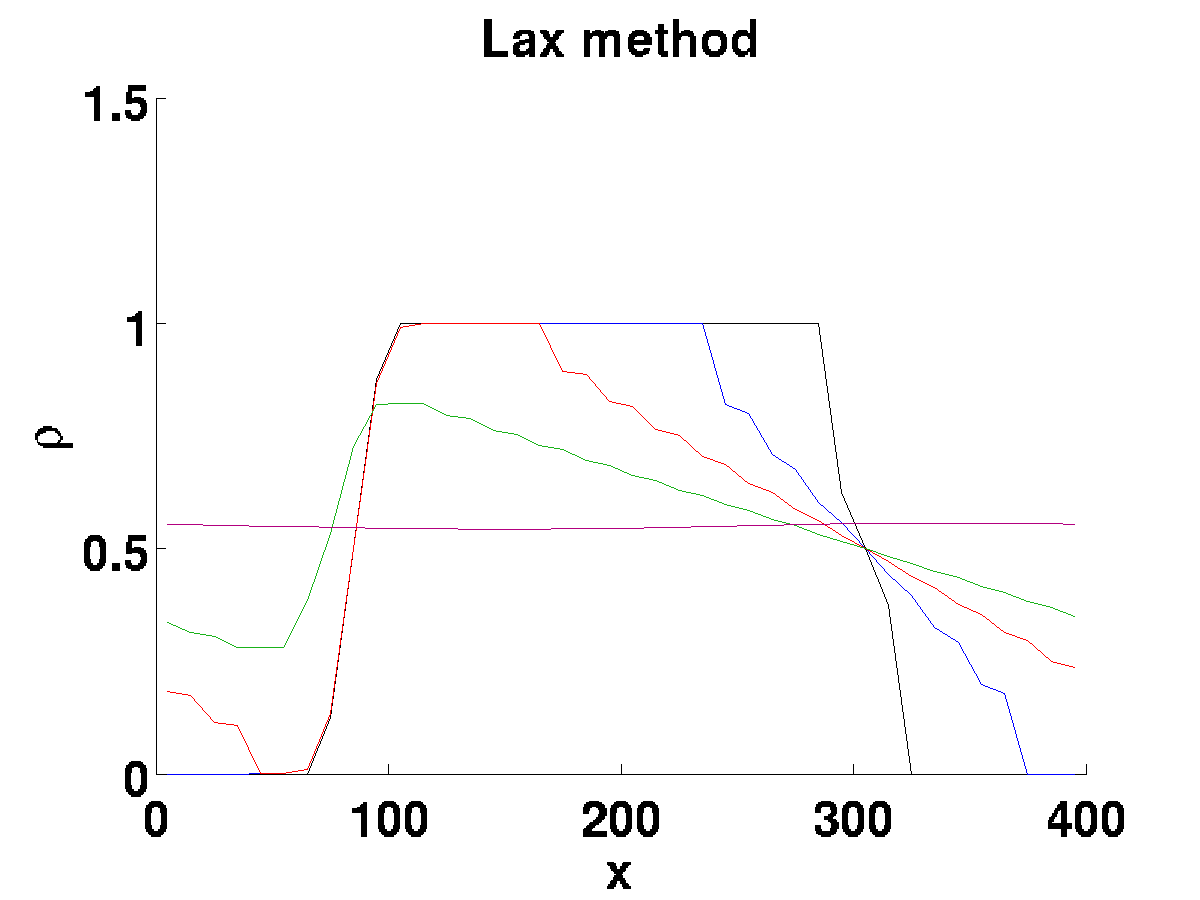
\includegraphics[width=\textwidth]{img/exc2_Lax_p}
	\caption{}
	\label{fig:exc2_Lax_p}
\end{subfigure}
\begin{subfigure}{.25\textwidth}
	\centering
	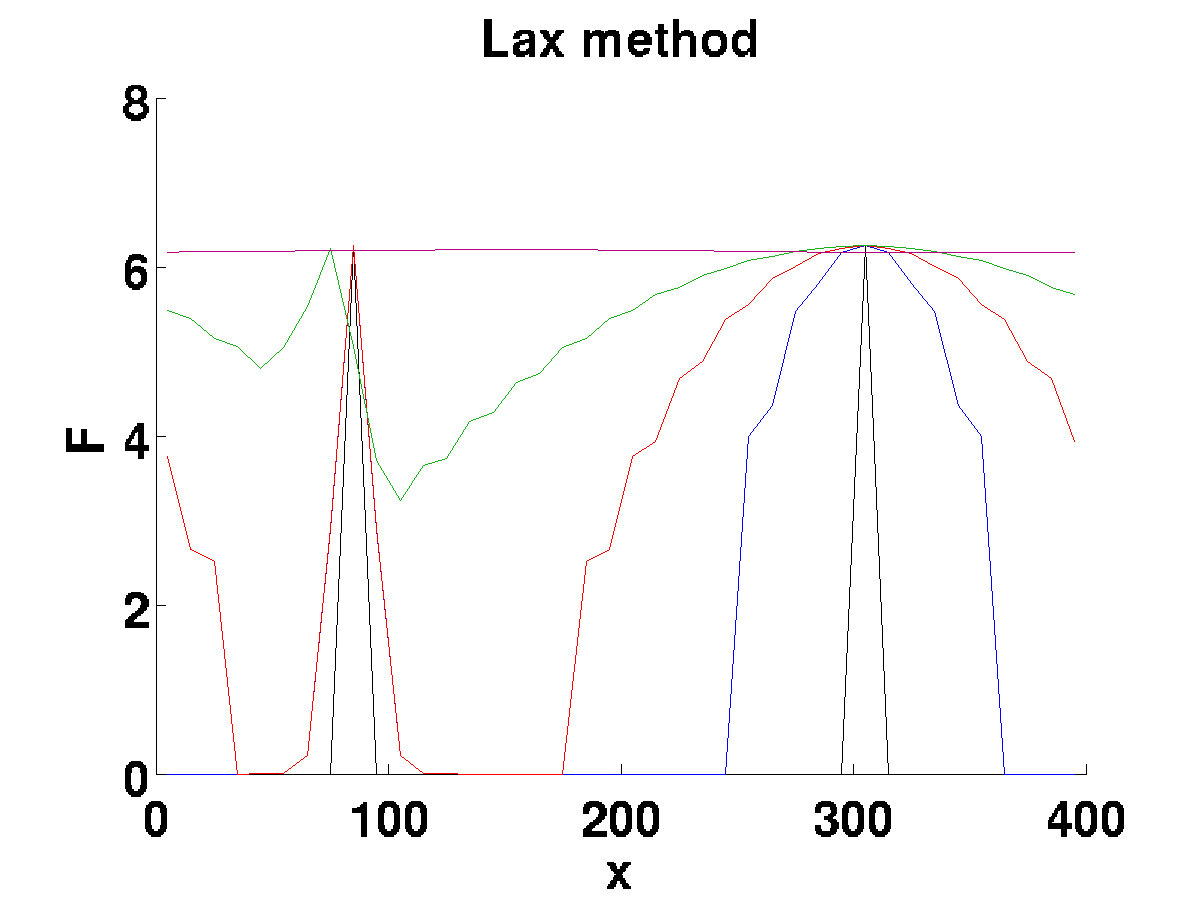
\includegraphics[width=\textwidth]{img/exc2_Lax_F}
	\caption{}
	\label{fig:exc2_Lax_F}
\end{subfigure}
\begin{subfigure}{.25\textwidth}
	\centering
	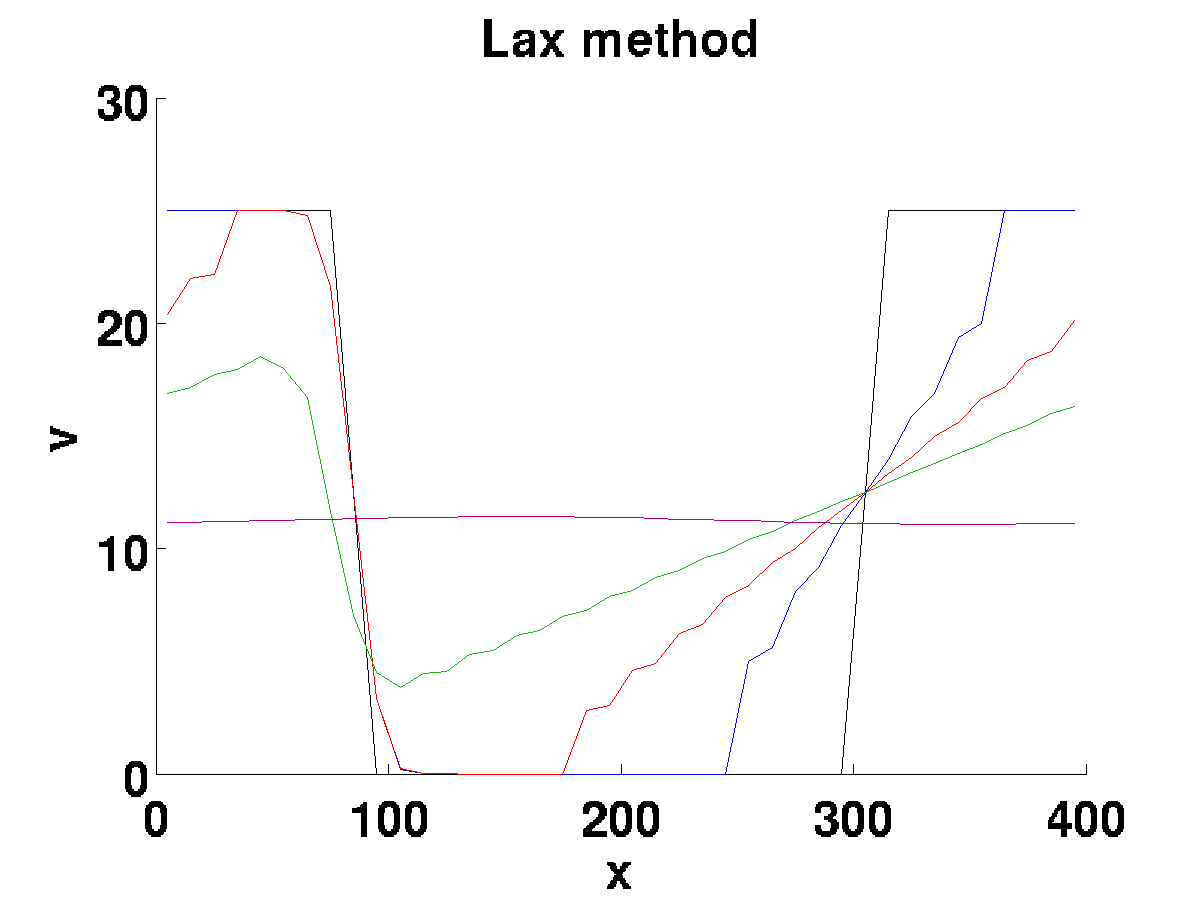
\includegraphics[width=\textwidth]{img/exc2_Lax_v}
	\caption{}
	\label{fig:exc2_Lax_v}
\end{subfigure}
\begin{subfigure}{.09\textwidth}
	\centering
	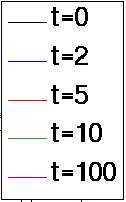
\includegraphics[width=\textwidth]{img/exc2_legend}
\end{subfigure}
\caption{Results of Burger's equation using the Lax scheme. (a) Plot of $\rho(x)$ versus position for different times. (b) Plot of $F(\rho(x))$ versus position for different times. (c) Plot of $v(\rho(x))$ versus position for different times.}
\label{fig:exc2_Lax_scheme}
\end{figure}

\begin{figure}[h!]
\begin{subfigure}{.25\textwidth}
	\centering
	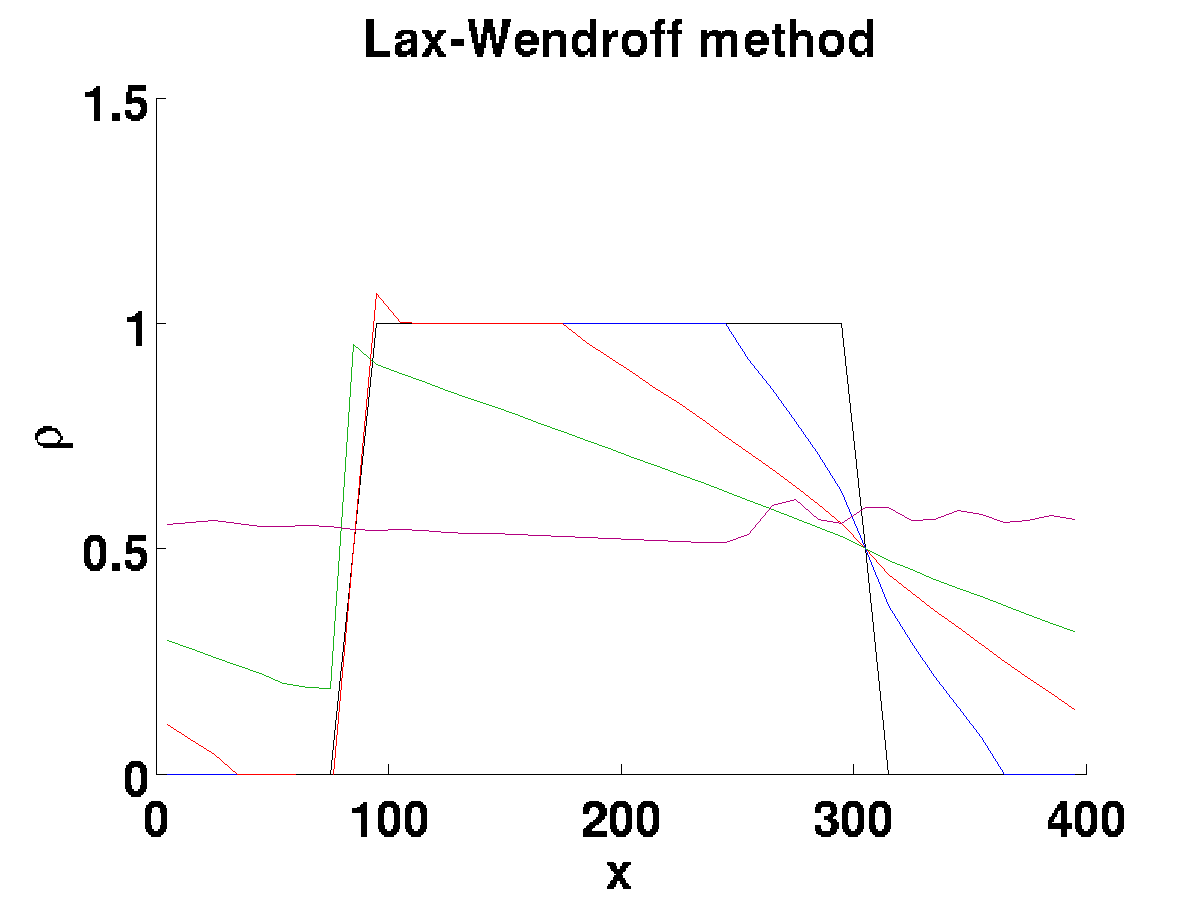
\includegraphics[width=\textwidth]{img/exc2_LW_p}
	\caption{}
	\label{fig:exc2_LW_p}
\end{subfigure}
\begin{subfigure}{.25\textwidth}
	\centering
	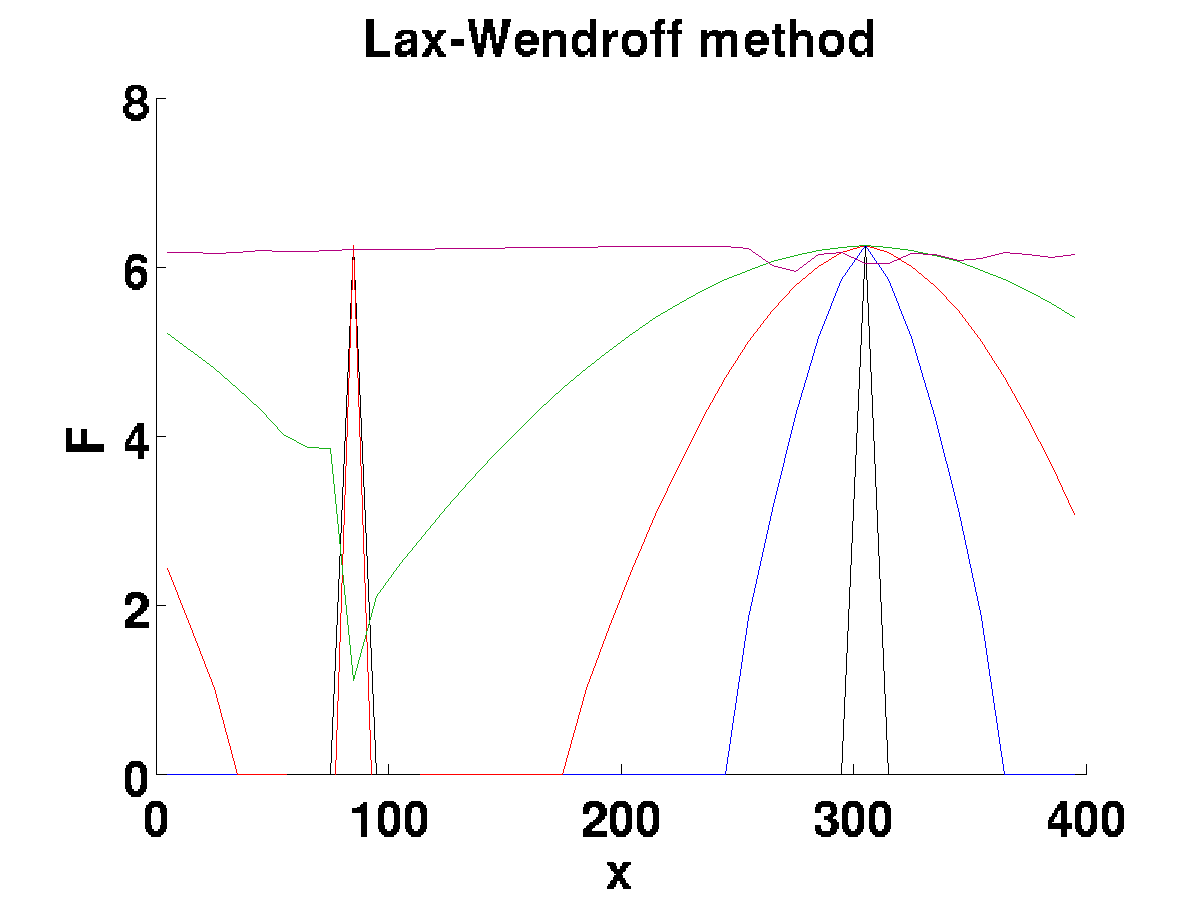
\includegraphics[width=\textwidth]{img/exc2_LW_F}
	\caption{}
	\label{fig:exc2_LW_F}
\end{subfigure}
\begin{subfigure}{.25\textwidth}
	\centering
	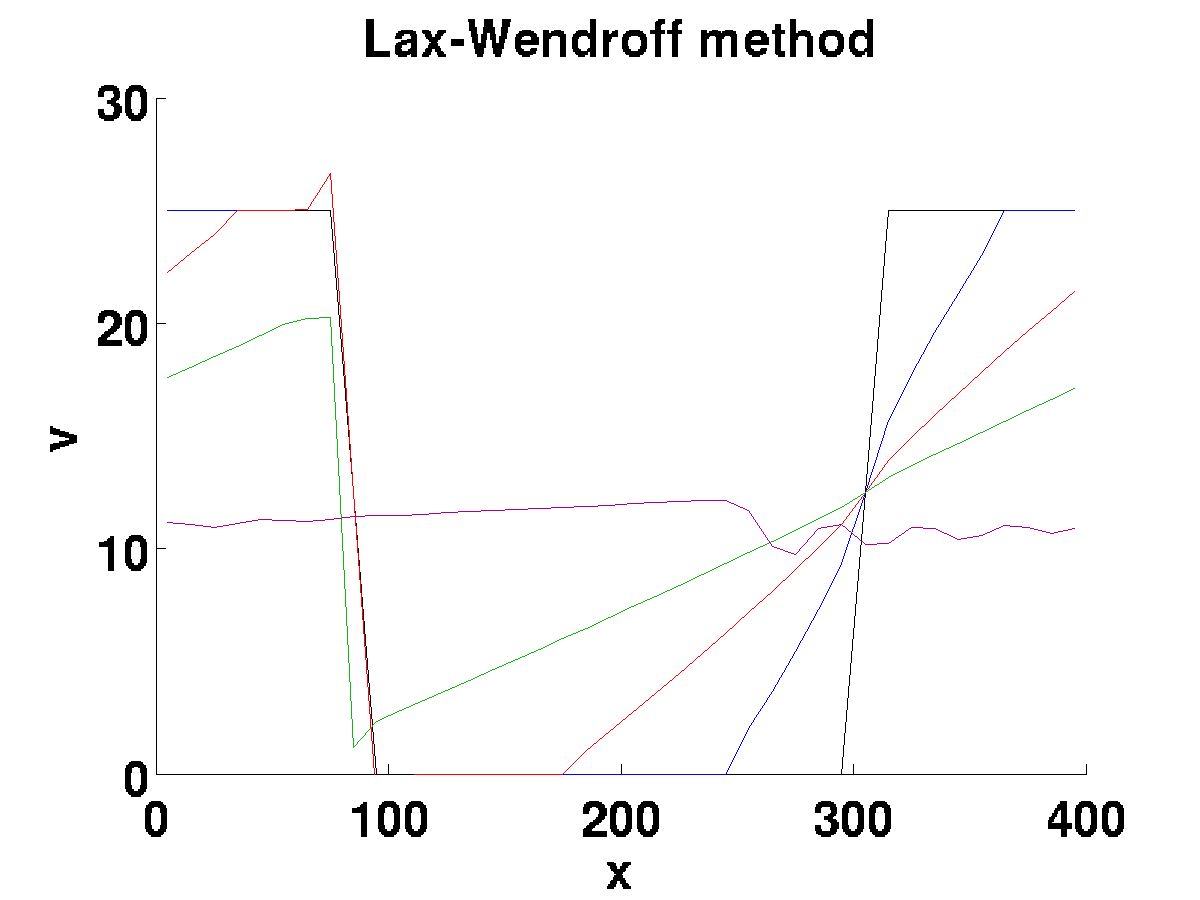
\includegraphics[width=\textwidth]{img/exc2_LW_v}
	\caption{}
	\label{fig:exc2_LW_v}
\end{subfigure}
\begin{subfigure}{.09\textwidth}
	\centering
	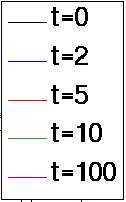
\includegraphics[width=\textwidth]{img/exc2_legend}
\end{subfigure}
\caption{Results of Burger's equation using the Lax-Wendroff scheme. (a) Plot of $\rho(x)$ versus position for different times. (b) Plot of $F(\rho(x))$ versus position for different times. (c) Plot of $v(\rho(x))$ versus position for different times.}
\label{fig:exc2_LW_scheme}
\end{figure}
\FloatBarrier

If increasing the time step $dt$ and keeping $dx$ fixed. For small enough times and not to large $dt$; the solution will no longer have this straight line between the last point where $\rho = \rho_m$ and $\rho = 0$ which is seen in the analytical solution, although otherwise evolving the right way. For larger $dt$ and larger times---the solution will not converge.
If decreasing the spatial step $dx$ and keeping $dt$ fixed. The errors are very similar to increasing $dt$ and keeping $dx$ fixed.
Comparing the two schemes, the Lax scheme seems to handle this error better than the Lax-Wendroff scheme.

